% Created 2026-09-25 Fri 21:43
% Intended LaTeX compiler: pdflatex
\documentclass[11pt]{article}

\usepackage[utf8]{inputenc}
\usepackage[T1]{fontenc}
\usepackage{graphicx}
\usepackage{longtable}
\usepackage{wrapfig}
\usepackage{rotating}
\usepackage[normalem]{ulem}
\usepackage{amsmath}
\usepackage{amssymb}
\usepackage{capt-of}
\usepackage{hyperref}
\usepackage[margin=1in]{geometry}
\usepackage{tabularx}
\usepackage{booktabs}
\usepackage[table]{xcolor}
\rowcolors{2}{white}{black!4}
\usepackage{float}
\usepackage{tikz}
\usetikzlibrary{positioning,arrows.meta,shapes.geometric,fit,backgrounds,calc}
\definecolor{rboxfill}{HTML}{EEF2F7}
\definecolor{rboxline}{HTML}{4A5568}
\definecolor{rrootfill}{HTML}{DBE4F0}
\definecolor{ranchorfill}{HTML}{FDF6E3}
\definecolor{rmutedfill}{HTML}{F4F4F5}
\definecolor{rmutedline}{HTML}{A0AEC0}
\definecolor{rmutedtext}{HTML}{555555}
\definecolor{rmutedline2}{HTML}{8A8F98}
\definecolor{rnafill}{HTML}{F5F5F5}
\definecolor{rnaline}{HTML}{BBBBBB}
\definecolor{rnatext}{HTML}{888888}
\tikzset{rbox/.style={rectangle, rounded corners=2pt, draw=rboxline, fill=rboxfill, minimum height=0.9cm, inner sep=6pt, align=center, font=\small}}
\tikzset{rroot/.style={rbox, fill=rrootfill}}
\tikzset{rmuted/.style={rbox, draw=rmutedline, fill=rmutedfill, text=rmutedtext}}
\tikzset{rnote/.style={rectangle, draw=rboxline, fill=ranchorfill, inner sep=5pt, align=center, font=\small}}
\tikzset{rna/.style={rectangle, draw=rnaline, fill=rnafill, text=rnatext, inner sep=5pt, align=center, font=\small}}
\tikzset{rdiamond/.style={diamond, draw=rboxline, fill=ranchorfill, align=center, font=\small, inner sep=2pt}}
\tikzset{redge/.style={-{Stealth[length=2.2mm]}, draw=rboxline, font=\scriptsize}}
\tikzset{rlabel/.style={font=\scriptsize, fill=white, inner sep=1pt, align=center}}
\author{Aseem Ratha}
\date{\today}
\title{Rashomon: A Desktop Environment Built on a Persistent Graph\\\medskip
\large Architecture Overview}
\hypersetup{
 pdfauthor={Aseem Ratha},
 pdftitle={Rashomon: A Desktop Environment Built on a Persistent Graph},
 pdfkeywords={},
 pdfsubject={},
 pdfcreator={},
 pdflang={English}}
\begin{document}

\maketitle
\setcounter{tocdepth}{2}
\tableofcontents

\clearpage

A desktop environment built around a persistent graph of information, rather than conventional applications and files. Anything encountered while computing (a webpage, a note, a conversation, a terminal session, a piece of media) can become a persistent, addressable thing in the graph. Programs become swappable, composable ways of encountering and manipulating that graph, rather than owners of their own private state.
\section{Core Model}
\label{sec:orgb7fc979}

\begin{center}
\begin{tabularx}{\textwidth}{lX}
\toprule
Term & Meaning\\
\midrule
\textbf{Rashomon} & the whole system\\
\textbf{Kernel} & the native process owning the graph, identity resolution, persistence, primitives, the component runtime, and the package manager\\
\textbf{Node} & the generic graph vertex. Every Node has a \textbf{role}: \texttt{entity} or \texttt{occurrence}\\
\textbf{Entity} & a Node with durable identity: a recurring page, a task, a topic, a browser profile\\
\textbf{Occurrence} & a Node representing one instance of running into something: this tab load, this shell session, this chat exchange. Weak/no identity of its own; always has exactly one \texttt{occurrence-of} edge to an Entity\\
\textbf{Edge} & a typed, directed link between two Nodes, carrying a timestamp and a confidence score\\
\textbf{Facet} & a declared way an Entity can be viewed or acted on (browser, notes, history, graph, terminal…)\\
\textbf{View} & one live, on-screen instance of a Facet being used right now. Facet = capability; View = an open instance of using it\\
\textbf{Component} & the sandboxed WASM binary implementing zero or more Facets' logic, and/or declaring, via its manifest, zero or more node/edge types it introduces (at least one of the two). Types are inert schema; only Facets carry behavior. Never implements a Primitive itself, only declares which ones it requires\\
\textbf{Native Backend} & the native, unsandboxed, kernel-bundled code that actually implements a given Primitive — e.g. CEF backing \texttt{rashomon:browser}, a PTY bridge backing \texttt{rashomon:process}. Part of the trusted kernel, not the installable Component ecosystem, despite sometimes shipping as a separate binary/process\\
\textbf{Window} & the OS-level surface a View is drawn in\\
\textbf{Primitive} & a host-implemented capability a Component can be granted access to (graph read/write, process spawn, browser control, network, storage…). Its backend is always a Native Backend, never an ordinary Component\\
\bottomrule
\end{tabularx}
\end{center}

One sentence: \textbf{the graph is made of Nodes (Entities and Occurrences) connected by Edges; an Entity exposes Facets, each implemented by a Component; opening a Facet creates a View, which is drawn in a Window; Components talk to the kernel only through Primitives.}

\begin{figure}[H]
\centering
\resizebox{\ifdim\width>\linewidth\linewidth\else\width\fi}{!}{%
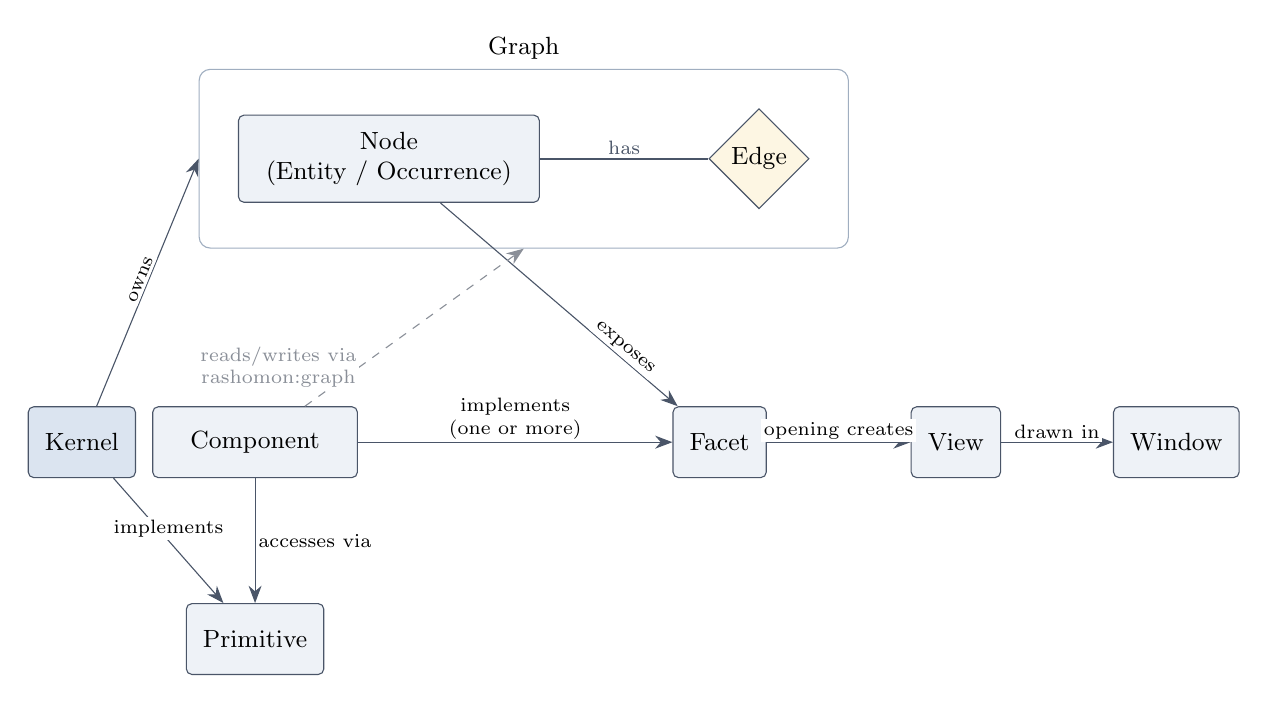
\begin{tikzpicture}
  \node[rroot] (kernel) at (0,0) {Kernel};
  \node[rbox, minimum width=2.6cm] (component) at (2.2,0) {Component};
  \node[rbox] (facet) at (8.1,0) {Facet};
  \node[rbox] (view) at (11.1,0) {View};
  \node[rbox] (window) at (13.9,0) {Window};
  \node[rbox] (primitive) at (2.2,-2.5) {Primitive};

  \node[rbox, text width=3.4cm] (nodebox) at (3.9,3.6) {Node\\(Entity / Occurrence)};
  \node[rdiamond] (edgebox) at (8.6,3.6) {Edge};

  \begin{pgfonlayer}{background}
    \node[draw=rmutedline, rounded corners=4pt, fit=(nodebox)(edgebox), inner sep=14pt, label={[font=\small]above:Graph}] (graphcluster) {};
  \end{pgfonlayer}

  \draw[rboxline, thick] (nodebox) -- (edgebox) node[rlabel, midway, above] {has};

  \draw[redge] (kernel) -- (graphcluster.west) node[rlabel, pos=0.5, above, sloped] {owns};
  \draw[redge] (kernel) -- (primitive) node[rlabel, midway, above] {implements};

  \draw[redge] (nodebox) -- (facet) node[rlabel, pos=0.75, above, sloped] {exposes};
  \draw[redge] (component) -- (facet) node[rlabel, midway, above, sloped] {implements\\(one or more)};
  \draw[redge] (facet) -- (view) node[rlabel, midway, above] {opening creates};
  \draw[redge] (view) -- (window) node[rlabel, midway, above] {drawn in};

  \draw[redge, dashed, draw=rmutedline2] (component) -- (graphcluster.south) node[rlabel, pos=0.25, left, text=rmutedline2] {reads/writes via\\rashomon:graph};

  \draw[redge] (component) -- (primitive) node[rlabel, midway, right] {accesses via};
\end{tikzpicture}%
}
\caption{Core concepts and how they relate: the Kernel, Nodes, Edges, Facets, Views, Components, and Primitives.}
\label{fig:concept-flow}
\end{figure}
\section{Layered overview}
\label{sec:org7625be3}

\begin{figure}[H]
\centering
\resizebox{\ifdim\width>\linewidth\linewidth\else\width\fi}{!}{%
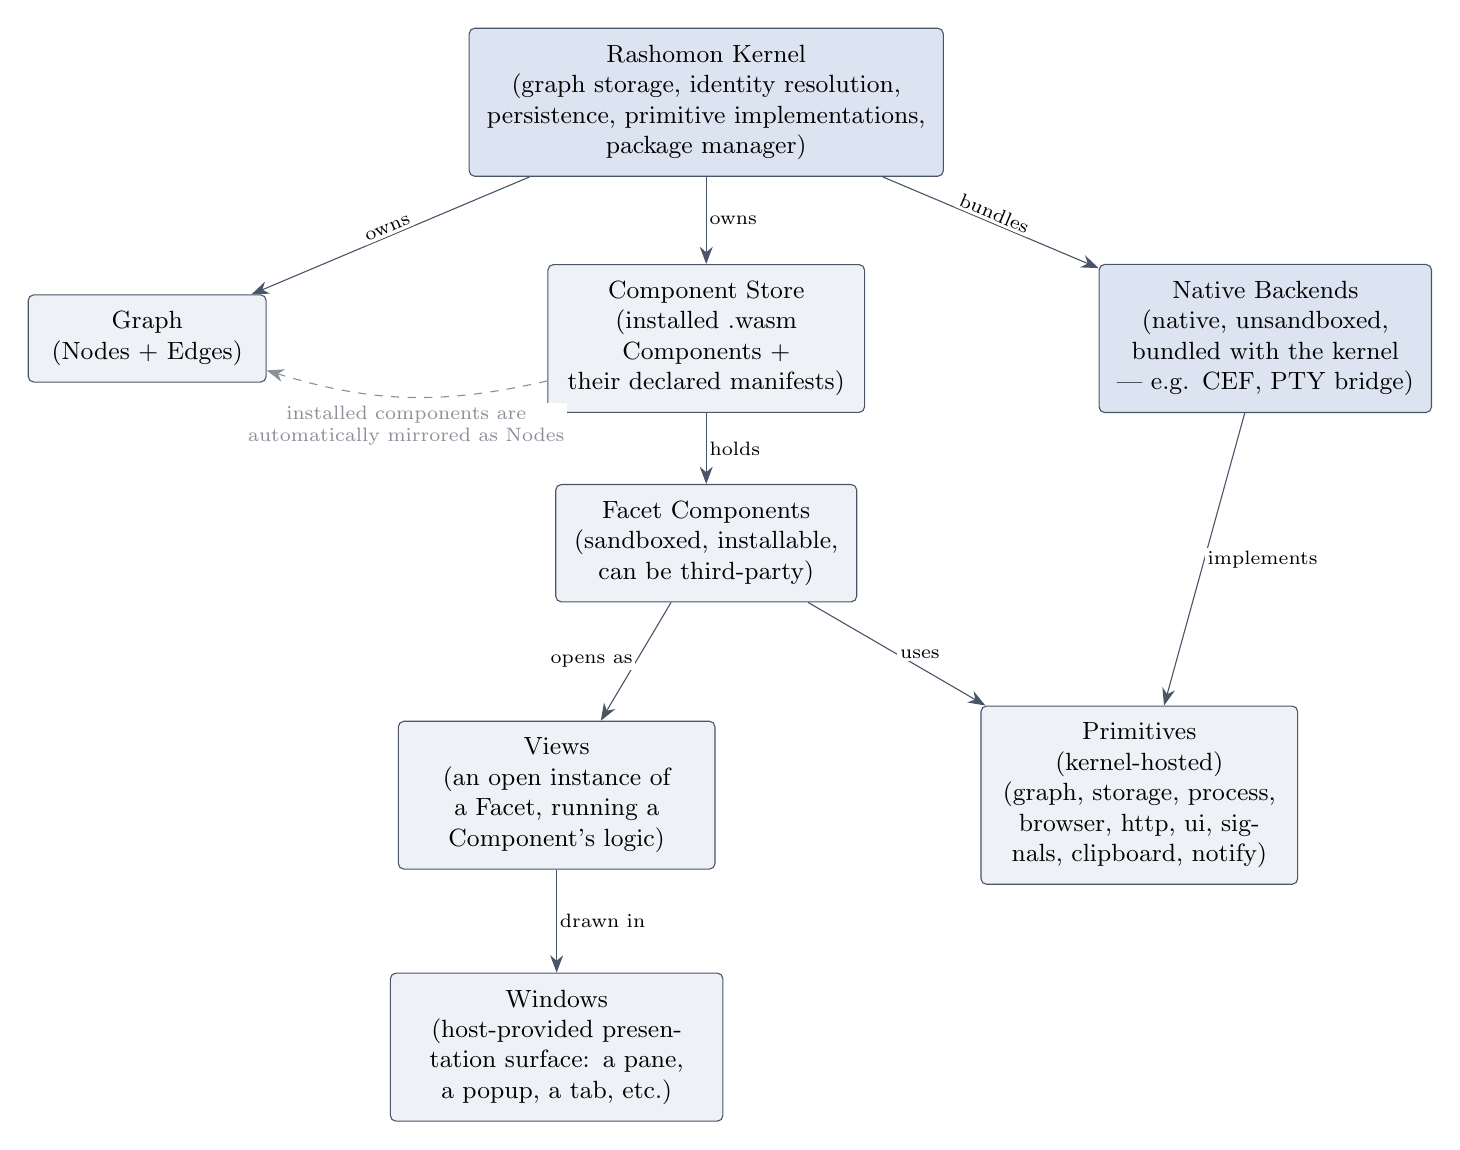
\begin{tikzpicture}
  \node[rroot, text width=5.6cm, align=center] (kernel) at (6.5,9.4)
    {Rashomon Kernel\\(graph storage, identity resolution,\\persistence, primitive implementations,\\package manager)};

  \node[rbox, text width=2.6cm] (graph) at (-0.6,6.4) {Graph\\(Nodes + Edges)};
  \node[rbox, text width=3.6cm] (compstore) at (6.5,6.4) {Component Store\\(installed .wasm Components +\\their declared manifests)};
  \node[rroot, text width=3.8cm] (compnative) at (13.6,6.4) {Native Backends\\(native, unsandboxed, bundled with the kernel --- e.g. CEF, PTY bridge)};

  \node[rbox, text width=3.4cm] (compfacet) at (6.5,3.8) {Facet Components\\(sandboxed, installable,\\can be third-party)};

  \node[rbox, text width=3.6cm] (primitives) at (12.0,0.6)
    {Primitives (kernel-hosted)\\(graph, storage, process, browser, http, ui, signals, clipboard, notify)};
  \node[rbox, text width=3.6cm] (views) at (4.6,0.6) {Views\\(an open instance of a Facet, running a Component's logic)};

  \node[rbox, text width=3.8cm] (windows) at (4.6,-2.6) {Windows\\(host-provided presentation surface: a pane, a popup, a tab, etc.)};

  \draw[redge] (kernel) -- (graph) node[rlabel, midway, above, sloped] {owns};
  \draw[redge] (kernel) -- (compstore) node[rlabel, midway, right] {owns};
  \draw[redge] (kernel) -- (compnative) node[rlabel, midway, above, sloped] {bundles};

  \draw[redge, dashed, draw=rmutedline2] (compstore) to[bend left=15] node[rlabel, pos=0.5, below=2pt, text=rmutedline2] {installed components are\\automatically mirrored as Nodes} (graph);

  \draw[redge] (compstore) -- (compfacet) node[rlabel, midway, right] {holds};

  \draw[redge] (compfacet) -- (primitives) node[rlabel, pos=0.5, right] {uses};
  \draw[redge] (compnative) -- (primitives) node[rlabel, pos=0.5, right] {implements};

  \draw[redge] (compfacet) -- (views) node[rlabel, pos=0.5, left] {opens as};
  \draw[redge] (views) -- (windows) node[rlabel, midway, right] {drawn in};
\end{tikzpicture}%
}
\caption{What the kernel directly owns (Graph, Component Store, Native Backends) versus what Facet Components provide on top (Views, Windows).}
\label{fig:layered-overview}
\end{figure}

Hosts (an extension, an Electron/CEF shell, eventually a browser fork) sit outside this entirely. They only provide Windows and route user input in. Swapping a host should never touch the graph, the primitives, or any Component.
\section{Nodes: roles vs. types}
\label{sec:org8af2230}

\texttt{entity} and \texttt{occurrence} are the only two \textbf{roles}, fixed by the kernel. This is what determines identity-resolution behavior and which structural edges apply. Concrete node \textbf{types} are open and component-defined, the same way Facets are.

A component's manifest registers the node types it introduces:

\begin{verbatim}
node-type shell-session {
    role: occurrence
    properties: { cwd: string, started-at: timestamp, exit-code: option<s32> }
}
\end{verbatim}

Types are namespaced (\texttt{rashomon:page}, \texttt{someauthor:shell-session}) so two components can't collide on the same name.

A type is deliberately just a shape: a \textbf{role} plus a \textbf{properties} block, nothing else. It has no attached behavior, so the kernel (and any Facet, whether or not it's the one that introduced the type) can always safely store and inspect it. All actual logic — rendering, proposing identity-resolution keys, interpreting edges — lives in Facets, never in a type declaration.

Because of that split, implementing a Facet, introducing a node type, and introducing an edge type are three \textbf{independent} things a Component's manifest can declare, not a package deal. A Component can be as small as a single new Facet over an \textbf{existing} type (a "kanban board" Facet grouping ordinary \texttt{thread} Entities by status, introducing no new type at all), or just a new type with no dedicated Facet (relying on a generic outline/thread view to show it), or a full feature bundling a new type with every Facet it needs. Here's the fuller end of that spectrum — a hypothetical chat Component that both introduces a type and implements several Facets over it:

\begin{figure}[H]
\centering
\resizebox{\ifdim\width>\linewidth\linewidth\else\width\fi}{!}{%
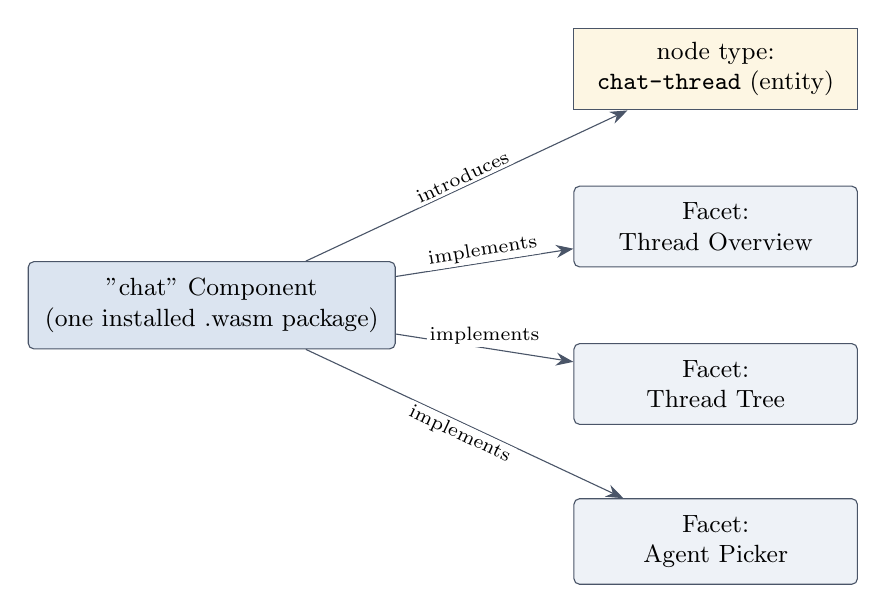
\begin{tikzpicture}
  \node[rroot, minimum width=4.4cm] (comp) at (0,0) {"chat" Component\\(one installed .wasm package)};

  \node[rnote, minimum width=3.6cm] (nodetype) at (6.4,3.0) {node type:\\\texttt{chat-thread} (entity)};
  \node[rbox, minimum width=3.6cm] (facet1) at (6.4,1.0) {Facet:\\Thread Overview};
  \node[rbox, minimum width=3.6cm] (facet2) at (6.4,-1.0) {Facet:\\Thread Tree};
  \node[rbox, minimum width=3.6cm] (facet3) at (6.4,-3.0) {Facet:\\Agent Picker};

  \draw[redge] (comp) -- (nodetype) node[rlabel, midway, above, sloped] {introduces};
  \draw[redge] (comp) -- (facet1) node[rlabel, midway, above, sloped] {implements};
  \draw[redge] (comp) -- (facet2) node[rlabel, midway, above] {implements};
  \draw[redge] (comp) -- (facet3) node[rlabel, midway, below, sloped] {implements};
\end{tikzpicture}%
}
\caption{One possible shape of a Component's declared surface --- a new node type plus every Facet it implements over it. A Component just as easily declares only one of these, or introduces no new type at all. Edge types (not pictured) work the same way.}
\label{fig:component-surface}
\end{figure}
\subsection{Built-in types (ship with the kernel)}
\label{sec:org6065743}

\begin{center}
\begin{tabularx}{\textwidth}{llX}
\toprule
Type & Role & Notes\\
\midrule
\texttt{thread} & entity & generic, no-schema; the default place to file anything with no more specific type\\
\texttt{page} & entity & a recurring web reference; identity resolved via URL + content similarity\\
\texttt{browser-context} & entity & a persistent browser profile/session identity\\
\bottomrule
\end{tabularx}
\end{center}
\subsection{Example third-party types}
\label{sec:org500f4f7}

\begin{center}
\begin{tabularx}{\textwidth}{llX}
\toprule
Type & Role & Notes\\
\midrule
\texttt{shell-session} & occurrence & one PTY-backed terminal run\\
\texttt{dev-task} & entity & optional richer entity a terminal component could define if generic \texttt{thread} isn't enough (tracks cwd/branch across sessions)\\
\texttt{chat-thread} & entity & optional richer entity a chat component could define if generic \texttt{thread} isn't enough (adds participant/topic keys for identity resolution)\\
\texttt{chat-exchange} & occurrence & one specific conversation instance under a \texttt{chat-thread}\\
\texttt{installed-component} & entity & the kernel's own package manager mirrors each installed Component as an ordinary Node, so it's queryable/browsable like anything else\\
\bottomrule
\end{tabularx}
\end{center}
\section{Edges}
\label{sec:orgc6e43b9}

\textbf{Structural} (kernel reasons about these directly):

\begin{itemize}
\item \texttt{Occurrence-of}: Occurrence → Entity. Mandatory, exactly one per Occurrence.
\item \texttt{Contains}: Entity → Entity. The outline/tree hierarchy (threads containing pages, pages containing markers). Single-parent by default, a strict tree rather than a DAG, so outline-style Facets can render it simply. A second relationship uses \texttt{references} instead.
\item \texttt{Supersedes} / \texttt{Diverged-from}: Entity → Entity. Produced by the identity-resolution ladder when a fuzzy match falls below the merge threshold, so a bad automatic call is correctable, not silently wrong.
\end{itemize}

\textbf{Typed, open} (kernel stores/queries generically; Components interpret):

\begin{itemize}
\item \texttt{References}: general "this points at that." An anchor is a specialization: \texttt{references} carrying an \texttt{anchor-spec} payload (quote + context, element descriptors, spatial position, or a media locator).
\item \texttt{Context-of}: Occurrence → Entity, for "this happened under this browser-context/profile."
\item \texttt{Derived-from}: provenance for generated content (a chat reply derived from the anchors in its context; a promoted note derived from a message).
\item \texttt{Related-to}: a deliberately weak, manual "these matter to each other." The intended mechanism for surfacing an Entity somewhere beyond its one \texttt{contains} parent, without relaxing \texttt{contains}'s single-parent tree. Undirected in practice, either side can create it, and an outline-style Facet is expected to render an Entity's \texttt{related-to} links as a secondary "Related" section alongside its primary \texttt{contains} children, not merged into the tree itself.
\end{itemize}

Edge types beyond this built-in set are open the same way node types are: declared in a Component's manifest, namespaced the same way (\texttt{rashomon:references}, \texttt{someauthor:blocks}), so a code-review Component could introduce its own \texttt{blocks} or \texttt{reviewed-by} edge type between issue Entities without touching the kernel.

Every edge carries a \textbf{timestamp} and a \textbf{confidence score} (1.0 for anything manual; a real number from the similarity check for automatic \texttt{supersedes} edges).
\section{Identity: entities and occurrences}
\label{sec:orgb040e6f}

Resolution is a per-occurrence matching problem, not a global definition of "what a webpage is." A \textbf{ladder}, run per occurrence against candidates a Facet's own matcher proposes:

\begin{enumerate}
\item \textbf{Strong key match}: a stable identifier (content hash, commit SHA, message ID). Exact match → same Entity, new version if content differs.
\item \textbf{Normalized-key match + similarity check}: e.g. a normalized URL. If an Entity already claims the key, diff new content against the last version. Above threshold → new version of the same Entity. Below threshold → new Entity, linked via \texttt{supersedes\textasciitilde{}/\textasciitilde{}diverged-from}.
\item \textbf{No match} → new Entity.
\end{enumerate}

Keys are typed and Facet-defined, not hardcoded in the kernel: a browser Facet proposes URL-based keys, a terminal Facet proposes directory+branch keys, a chat Facet proposes participant+topic keys. Every merge/split is logged and reversible.
\section{Primitives}
\label{sec:orge356058}

A fixed, versioned WIT package every Component's \textbf{world} is composed from. Semver'd independently of the kernel's internals. This is the contract a future maintainer only needs to keep stable, not every Facet ever published.

\begin{itemize}
\item \texttt{rashomon:graph}: read/write Nodes and Edges; propose-match calls for the identity ladder.
\item \texttt{rashomon:storage}: a sandboxed scope per Component.
\item \texttt{rashomon:process}: spawn/manage OS processes via a \texttt{resource process} handle (stream in/out, resize, signal, wait). Its Native Backend owns the actual \texttt{exec()}; a Component never gets a raw syscall.
\item \texttt{rashomon:browser}: \texttt{resource browser-context} (a persistent profile: cookies, cache, logins, itself represented as a \texttt{browser-context} Entity) and \texttt{resource browser-tab} (navigate, DOM snapshot, inject script, anchor, downloads) — a low-level handle for one browsing surface, not to be confused with a Core Model \textbf{View}. Backed by CEF as its Native Backend; never embedded in WASM itself (too heavy, needs native GPU/windowing).
\item \texttt{wasi:http}: standard, reused rather than wrapped.
\item \texttt{rashomon:ui}: a render-surface contract: a Component hands back a description of what to draw; the host draws it.
\item \texttt{rashomon:signals}: subscribe to graph changes, timers, lifecycle.
\item \texttt{rashomon:clipboard} / \texttt{rashomon:notify}: small, obviously-scoped.
\end{itemize}

This set is closed, not extensible the way Facets and node/edge types are: a Component can only ever \textbf{require} a Primitive (declare it as an import), never implement one. Every Primitive's actual backend is a Native Backend, native and unsandboxed by necessity, since a sandboxed WASM binary has no ambient authority to spawn processes or drive a browser engine on its own. Some Native Backends are inline in the kernel binary itself; others (CEF, a PTY bridge) ship as separate native processes for isolation, but both are part of the trusted kernel distribution, not the installable Component ecosystem. Whether a narrower, genuinely lower-risk subset of Primitives (\texttt{rashomon:clipboard}, \texttt{rashomon:notify}) should ever open up to third-party-supplied backends is an open question, not the current design — it would mean auditing a very different threat model than "sandboxed Component with a declared world."

A Component's declared world (its imports) is static and inspectable before install: the permission-prompt story, shown the way an extension's requested permissions are shown today.

\textbf{Decide \texttt{rashomon:process} and \texttt{rashomon:browser} against a real Facet} that needs them, not in the abstract. Designing a capability before the first consumer exists is a common way these interfaces end up wrong.
\section{Self-hosting}
\label{sec:org61cdb90}

State lives in the \textbf{graph}, not inside a Component instance. A Component is closer to a stateless request handler over persistent Nodes than a live object with private state. That's what makes \textbf{hot-swap} (replace a running instance with a freshly compiled one) practical, even though true Lisp/Smalltalk-style \textbf{hot-edit} (mutating running code in place) isn't available to a compiled, sandboxed WASM binary.

The core design rule: \textbf{anything the kernel needs to show or manage about itself must first be representable as Nodes and Edges}, so managing it can be delegated to an ordinary Component. The node-type registry browser, the package manager, and the outline/thread view should all be installed Components from day one (not privileged native UI), or the system never actually becomes self-hosting later.

A REPL/scripting Facet is a plausible later addition (Nyxt's Lisp REPL, Emacs's \texttt{eval-buffer} are the precedent) but is \textbf{deferred}, not required while Components can already be written in any supported language, and worth designing only once the friction of not having one is concrete.
\section{Packaging and distribution}
\label{sec:org498caaf}

A package = one \texttt{.wasm} file + a manifest declaring node types, Facets, edge types, and required primitives, the direct equivalent of a \texttt{.vsix}.

\begin{itemize}
\item \textbf{Local dev loop:} load straight from a directory (VS Code's "install from location" pattern), skipping the registry round-trip while iterating.
\item \textbf{Distribution:} skip \texttt{warg\textasciitilde{}/\textasciitilde{}wa.dev} for now (still early) in favor of a signed-manifest index hosted on GitHub, browsed through an Extensions Facet (itself a Component) that shows requested capabilities before install: fetch, verify hash/signature, unpack, register. No config file editing, ever, for the install path itself.
\item Revisit \texttt{warg} once it matures; the manifest format should be designed so migrating onto it later doesn't require re-authoring packages.
\end{itemize}
\section{Concurrency}
\label{sec:org43962ea}

\begin{itemize}
\item \textbf{Across Views/Components:} each active View gets its own Wasmtime \texttt{Store}. I/O-bound work (watchers, streaming chat, browser events) runs as async tasks sharing an executor (Wasmtime's component-model-async support). CPU-bound work dispatches its \texttt{Store}'s call onto a worker thread so it doesn't stall the executor.
\item \textbf{Within a single Component:} true in-guest multithreading needs the WebAssembly "shared-everything-threads" proposal, which is still immature. \textbf{Don't build around it.} Instead, a Component that needs real parallel compute calls a \textbf{primitive} backed by a Native Backend (multithreaded Rust on the host side) and awaits the result. This is the same host-mediated pattern as \texttt{rashomon:process} and \texttt{rashomon:browser}.
\end{itemize}
\section{Tech stack}
\label{sec:org1f1e867}

\begin{itemize}
\item \textbf{Kernel:} Rust.
\item \textbf{WASM runtime:} Wasmtime, the Bytecode Alliance reference implementation, furthest along on the Component Model and WASI Preview 2.
\item \textbf{Browser primitive Native Backend:} CEF via \texttt{cef-rs} (the Tauri-maintained fork), actively tracked against current Chromium releases, ships its own binary-download and app-bundling tooling.
\item \textbf{Component authoring:} any language with WIT bindings. Rust (\texttt{cargo-component}) is most mature; JS (\texttt{jco}), Python (\texttt{componentize-py}), and Go (TinyGo) are workable; C/C++ guest support is real but currently the least polished.
\item \textbf{UI:} HTML-based, described by Components through \texttt{rashomon:ui} and drawn by the host, not native per-toolkit UI code.
\end{itemize}
\section{Worked example}
\label{sec:org3c9eda5}

A thread called \textbf{"researching CRISPR delivery methods"}:

\begin{figure}[H]
\centering
\resizebox{\ifdim\width>\linewidth\linewidth\else\width\fi}{!}{%
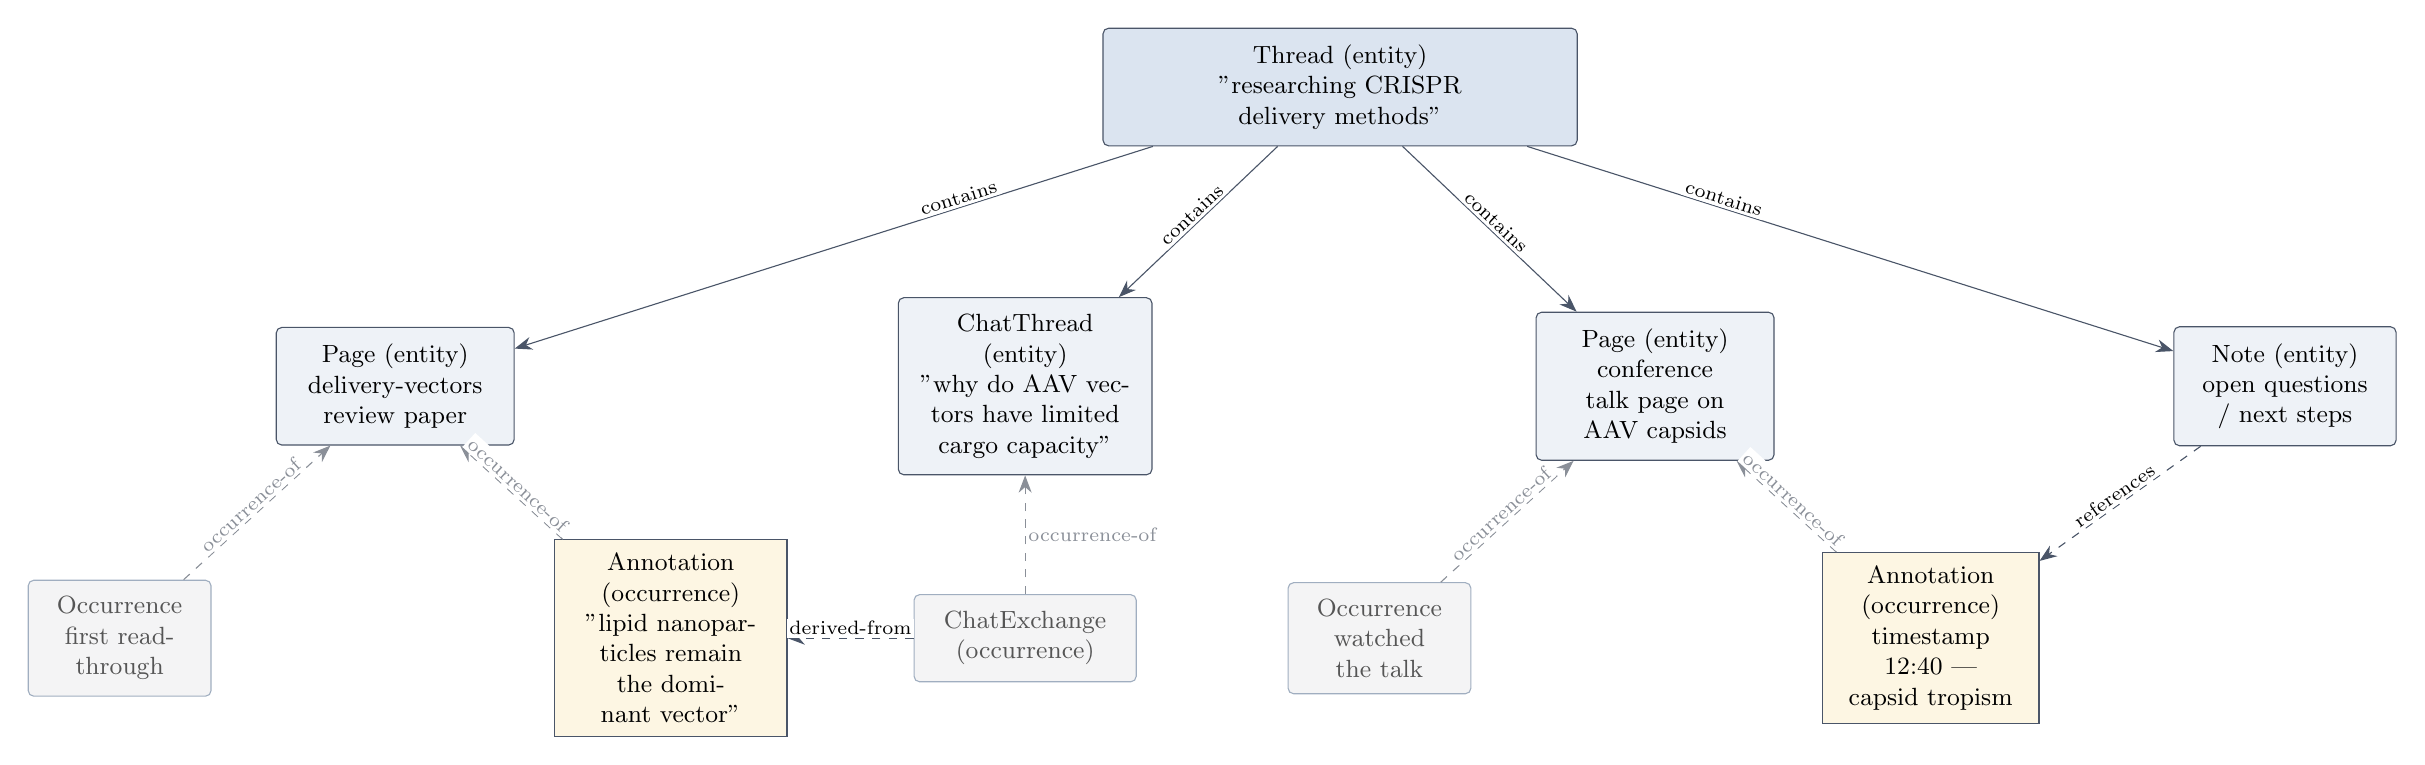
\begin{tikzpicture}
  \node[rroot, text width=5.6cm] (thread) at (12,8.8) {Thread (entity)\\"researching CRISPR delivery methods"};

  \node[rbox, text width=2.6cm] (page1) at (0,5) {Page (entity)\\delivery-vectors review paper};
  \node[rmuted, text width=1.9cm] (occ1) at (-3.5,1.8) {Occurrence\\first read-through};
  \node[rnote, text width=2.6cm] (anchor1) at (3.5,1.8) {Annotation (occurrence)\\"lipid nanoparticles remain\\the dominant vector"};

  \node[rbox, text width=2.8cm] (chatthread) at (8,5) {ChatThread (entity)\\"why do AAV vectors have limited cargo capacity"};
  \node[rmuted, text width=2.4cm] (chatexch) at (8,1.8) {ChatExchange (occurrence)};

  \node[rbox, text width=2.6cm] (page2) at (16,5) {Page (entity)\\conference talk page on AAV capsids};
  \node[rmuted, text width=1.9cm] (occ2) at (12.5,1.8) {Occurrence\\watched the talk};
  \node[rnote, text width=2.4cm] (anchor2) at (19.5,1.8) {Annotation (occurrence)\\timestamp 12:40 --- capsid tropism};

  \node[rbox, text width=2.4cm] (note) at (24,5) {Note (entity)\\open questions / next steps};

  \draw[redge] (thread) -- (page1)      node[rlabel, pos=0.3, above, sloped] {contains};
  \draw[redge] (thread) -- (chatthread) node[rlabel, midway, above, sloped] {contains};
  \draw[redge] (thread) -- (page2)      node[rlabel, midway, above, sloped] {contains};
  \draw[redge] (thread) -- (note)       node[rlabel, pos=0.3, above, sloped] {contains};

  \draw[redge, dashed, draw=rmutedline2] (occ1) -- (page1) node[rlabel, midway, above, sloped, text=rmutedline2] {occurrence-of};
  \draw[redge, dashed, draw=rmutedline2] (anchor1) -- (page1) node[rlabel, midway, above, sloped, text=rmutedline2] {occurrence-of};
  \draw[redge, dashed, draw=rmutedline2] (chatexch) -- (chatthread) node[rlabel, midway, right, text=rmutedline2] {occurrence-of};
  \draw[redge, dashed, draw=rmutedline2] (occ2) -- (page2) node[rlabel, midway, above, sloped, text=rmutedline2] {occurrence-of};
  \draw[redge, dashed, draw=rmutedline2] (anchor2) -- (page2) node[rlabel, midway, above, sloped, text=rmutedline2] {occurrence-of};

  \draw[redge, dashed] (chatexch) -- (anchor1) node[rlabel, midway, above] {derived-from};
  \draw[redge, dashed] (note) -- (anchor2) node[rlabel, midway, above, sloped] {references};
\end{tikzpicture}%
}
\caption{A thread ("researching CRISPR delivery methods") and the Nodes/Edges filed under it.}
\label{fig:worked-example}
\end{figure}
\section{Open / deferred decisions}
\label{sec:org9a0b4e0}

\begin{itemize}
\item Whether \texttt{rashomon:process} ships in v1 or waits for the first real terminal Facet to design against.
\item Same question for \texttt{rashomon:browser}'s multi-context isolation: build single-context/single-view first.
\item Scripting/REPL Facet: deferred until the friction is concrete.
\item \texttt{warg} adoption: revisit once it's past its early stage.
\item Whether \texttt{contains} should ever allow multiple parents: currently single-parent by design. Multi-parent would cost real complexity: an ambiguous canonical location/breadcrumb for outline Facets, messier move and delete semantics (reference-counting instead of a clean single reparent or delete), and the risk of accidentally-created cycles in what's meant to be a strict hierarchy. The likely resolution isn't relaxing \texttt{contains} itself but leaning on \texttt{related-to}: an Entity genuinely relevant to a second Thread gets a \texttt{related-to} edge to it, and outline Facets render that as a secondary "Related" section, most of the multi-homing benefit without sacrificing a single canonical home.
\end{itemize}
\end{document}
